\scanpage{8}
\mspage{2}
On a une application bijective
\[
\vec A\overset{\mathrm{rd}}{\simeq}A_{\unsure{*}}(C)\quad\text{ens des arêtes de }C
\]
\[
\vec a\longmapsto\text{``côté \deleted{gauche}\inserted{droite} de $\vec a$''}
\]
et chaque arête de $C$ est orientée de façon naturelle via cette application. Donc l'ens. des \uline{arcs} $\vec A(C)$ s'identifie à
\[
A(C)\times\{\pm1\}\simeq\vec A\times\{\pm1\},
\]
et l'involution $\sigma_0^C$ (passage à l'arête opposée) s'identifie à $\deleted{\unsure{\sigma}}\unsure{\sigma_\Gamma|\mathrm{id}}\times\tau$, $\tau$ la transposition de $\pm1$. Reste à définir $\sigma_1^C$, on le définit séparément sur
\[
\underbrace{\vec A\times\{+1\}}_{=\mathrm{rg}(\vec A)}=\vec A(C)_+
\]
et sur
\[
\underbrace{\vec A\times\{-1\}}_{\mathrm{rd}(\vec A)}=\vec A(C)_-.
\]
On a :
\margin{\uline{NB} $\vec A(C)$ est une \uline{\unsure{réunion|orientation}} des contours}
\figure{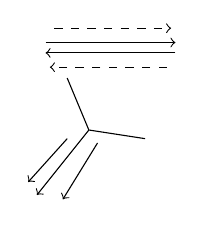
\begin{tikzpicture}[scale=.55]
\draw[->] (0,.12)--(3,.12);\draw[->] (3,-.12)--(0,-.12);\draw[dashed,->] (.2,.45)--(2.9,.45);\draw[dashed,->] (2.8,-.45)--(.1,-.45);
\draw (1,-1.9)--(.5,-.7) (1,-1.9)--(2.3,-2.1);\draw[->] (1,-1.9)--(-.2,-3.4);\draw[->] (.5,-2.1)--(-.4,-3.1);\draw[->] (1.2,-2.2)--(.4,-3.5);
\end{tikzpicture}}
\margin{$\unsure{A}$}
\[
\boxed{\begin{aligned}
\sigma_1^C(\mathrm r\deleted{\unsure{\mathrm g}}\mathrm d(\vec a))&=\deleted{\unsure{\mathrm{rd}}}\mathrm{rg}(\rho_\Gamma^{-1}(\vec a))=\sigma_0^C\mathrm{rd}(\rho_\Gamma(\vec a))\\
\sigma_1(\mathrm r\deleted{\unsure{\mathrm d}}\mathrm g(\vec a))&=\mathrm r\deleted{\unsure{\mathrm g}}\mathrm d(\rho_\Gamma^{\deleted{\unsure{-1}}}(\vec a))\deleted{\unsure{=\sigma_0^C}}
\end{aligned}}
\]
\[
\deleted{\rho_{\unsure{s}}(\vec a)=}
\left\{\begin{aligned}
\rho_C(\mathrm{rd}\vec a)&=\mathrm{rd}(\rho_\Gamma^{\deleted{\unsure{-1}}}(\vec a))\\
\rho_C(\mathrm{rg}\vec a)&=\unsure{\mathrm g|\mathrm{rg}}(\rho_\Gamma^{-1}\deleted{\unsure{\sigma_\Gamma}}\vec a))
\end{aligned}\right.
\]
\margin{\uline{NB} La définition des \uline{contours} \uline{orientés} $C$ ne dépend que de $\vec A$ muni de $\unsure{\rho_C|\rho_\Gamma}$ (à l'exclusion de $\sigma_0$)}
\figure{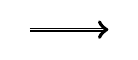
\begin{tikzpicture}\draw[double,->] (0,0)--(1,0);\end{tikzpicture}}

\unsure{Le} contour $C$ : \unsure{incidé} \unsure{sens} des \unsure{Aristyp.}

a) $C$ est orienté (``sens direct autour de $\Gamma$'')
\deleted{\deleted{\unsure{C}} $C'$ \unsure{par} ``\unsure{juxtaposition}'' i.e. \unsure{chaque} \inserted{(tient compte de $\unsure{o}$)} \unsure{est} \unsure{orientée}, soit la donnée d'une application \unsure{canonique}
\[
\vec A(C)'_+\subset\vec A(C),
\]
(``\unsure{plages} \unsure{topologiques}'') : \unsure{la} \unsure{unique} \unsure{p.}
\[
A(C)\longrightarrow\pm1
\]
\unsure{donnant} la valeur \unsure{$+1$ et $-1$} sur les deux \unsure{côtés}.}

\margin{i.e. on a\par
$\vec A=\vec A(C)_+\subset\vec A(C)$\par
ou\par
$\sigma_0\vec A=\vec A(C)_-$\par
$\sigma_1\vec A=\vec A(C)_-$}
Donc
\[
\left\{\begin{aligned}
\vec A(C)&\simeq\uline{\vec A(C)_+}\times\{\pm1\}\\
\sigma_0^C&\simeq\mathrm{id}\times\tau
\end{aligned}\right.
\]
La donnée de $\sigma_1^C$ revient à celle d'une permutation
\[
\rho_C=\{\vec a\longrightarrow\sigma_1^C(\sigma_0^C(\vec a))\}\quad\text{sur }\vec A.
\]
b) On a une involution, sans pts fixes $\sigma_\Gamma$ sur l'ens \deleted{\unsure{des}} des côtés de $C$, qui s'identifie à :
\[
\vec A=\vec A(C)_+.
\]
\mspage{7}
